\section{Background}
\label{sec:background}

\subsection{Conv2D tensor operation}
The \emph{Conv2D} tensor operation is described in \Equ{eq:conv2D}, where $h$ is the input feature map, $W$ is the convolution kernel (known as filter), and $b$ is the bias for the output feature map\cite{goodfellow2016deep}. We denote \emph{Conv} as \emph{Conv2D} operator.
\begin{eqnarray} \label{eq:conv2D}
Conv\left(W,h\right)_{i,j,o}=\sum_{k,l,m}^{K,L,M} h_{(i+k,j+l,m)} W_{(o,k,l,m)}+b_{o}
\end{eqnarray}

\subsection{Floating-point Number Representation}
The representation of every numerical value, in any number system, is made up of an integer and a fractional part. The border that delimits them is called the radix point. The fixed-point format for representing numeric values derives its name from the fact that in this format, the base point is fixed at a certain position. For integer numbers, this position is at the right of the least significant digit.

In scientific computation, it is often necessary to represent very large and very small values. This is difficult to achieve using the fixed point format because the bit width required to maintain both the desired precision and the desired range are very large. In such situations, floating-point formats are used to represent real numbers. Floating-point formats resemble scientific notation, such as $-5.90007\times10^{17}$. Each floating-point number can be divided into three fields: sign $s$, exponent $e$, and fraction $f$. Using the binary number system, it is possible to represent any floating-point number as:

\begin{eqnarray} \label{eq:float}
(-1)^{s} \times 1.f \times 2^{e-bias}
\end{eqnarray}

In this representation the exponent is biased, this means that the stored value is offset from 0 by a given value depending on the bit width of the exponent field in the particular format. The fraction represents the portion of the mantissa to the right of the radix point.

There is a natural trade-off between reduced bit widths requiring fewer hardware resources and larger bit widths providing higher precision. Within a given total bit width, it is possible to assign various combinations of bit widths to the exponent and fraction fields, with wider exponents resulting in a higher range and wider fractions resulting in better precision.

The most widely used format for floating-point arithmetic is the IEEE 754 standard \cite{ieee1985ieee}. This standard details basic and extended floating-point formats, each in single and double precision bit widths. The IEEE single-precision format (32-bit) is the same as shown in \Equ{eq:float} with $bias$ = 127, 8 bits for the exponent and 23 bits for the fraction. In IEEE format, the numbers are normalized and only the fractional part is stored.

Bit widths much smaller than those specified in the IEEE 754 standard are often sufficient to provide the desired precision. Reduced bit width implementations require fewer hardware resources and therefore allow low-power implementations than using the full IEEE standard format. In custom hardware designs, it is possible to have full control and flexibility over the exact floating-point format implemented. In this article, we focus on the 6-bit floating-point representation for the convolution parameters.

\begin{figure}[h!]
	\centering
	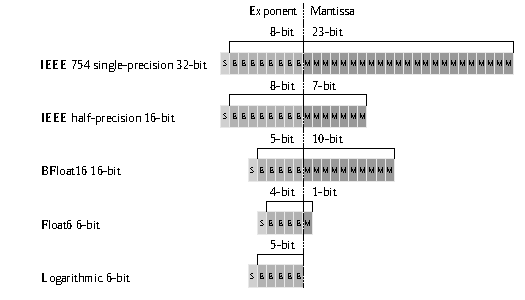
\includegraphics[width=1\columnwidth]{../figures/power_breakdown/floating_point.pdf}
	\caption{Floating-point number representation.}
	\label{fig:floating}
\end{figure}